\documentclass[../../main.tex]{subfiles}

\begin{document}

\begin{figure}[H]
    \centering
    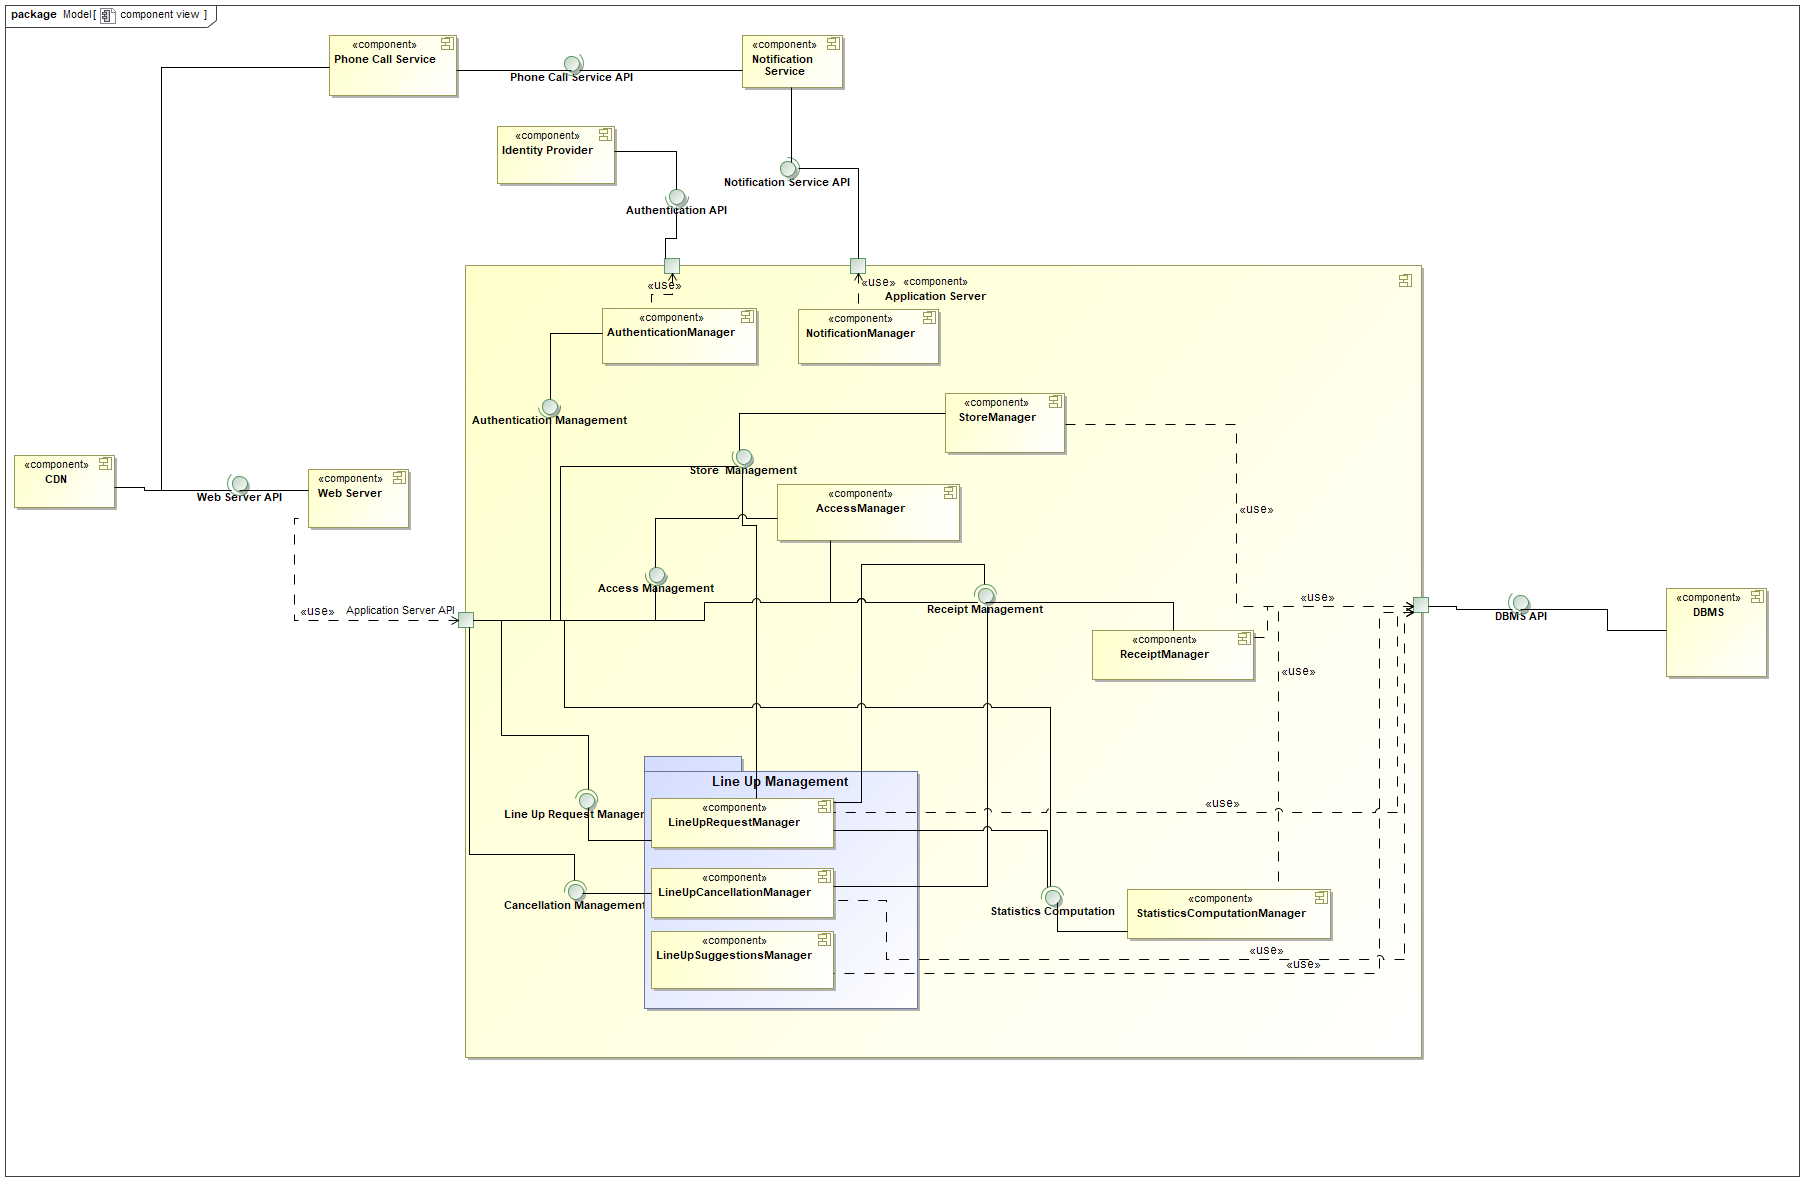
\includegraphics[width=\textwidth]{component_view.png}
    \caption{
        Component diagram
    }
\end{figure}

The component diagram above presents a general view of the application. 
The image describes the application server and its components with the highest level of detail, 
as developers will have to implement the business logic themselves. The other nodes in the system, as well as the services, 
are depicted more abstractly. Developers of the project might choose to use commercial off the shelf solutions 
to provide those APIs, thus losing control on the internal components, but accelerating the development.


The main components in the application server, providing all the business logic in CLup, are:

\begin{description}
    
    \item[AccessManager] The access manager encapsulates the business logic necessary to manage both entries in and exits from the store. 
    This component interacts with the ReceiptManager both to validate the entrance and to record the departure from the store. 
    The access manager also unlocks the turnstiles if the receipt is valid. 

    \item[AuthenticationManager] The authentication manager handles authentication for the functionalities of the 
    system reserved to store managers and store assistants. The authentication manager delegates the verification of the 
    identity of the user to an external provider.

    \item[LineUpCancellationManager] The LineUpCancellation manager is in charge of the cancellation process for 
    a reserved time slot. The change is performed in the persistent storage of the database and the receipt is marked as 
    invalid through the interface provided by the ReceiptManager.
    
    \item[LineUpRequestManager] The LineUpRequestManager implements the business logic behind the lining up to the store. 
    The LineUpRequestManager is in charge of both immediate queueing and reservations, 
    checking the availability of the time slot in the given store from StoreManager and then interfacing with the 
    ReceiptManager to generate the receipt to enter the store. During the process, the component also retrieves 
    statistics from the StatisticsComputationManager.

    \item[LineUpSuggestionsManager] The LineUpSuggestionsManager is in charge of finding alternatives to the time slot and 
    store requested by the customer if they are not available. To do so, it interacts with the database retrieving data 
    regarding the queues to other stores.

    \item[NotificationManager] The NotificationManager is in charge of sending notifications to customers when their visit's time is near, 
    according to their geographical distance from the store. This component is the only one not implementing a typical 
    client-server interaction in the application server. The push behaviour in the notification management is 
    achieved by using the interfaces provided by notification services.

    \item[ReceiptManager] The ReceiptManager is in charge of the operations performed on the receipt by updating its 
    state in the database. CRUD operations on the receipt are performed through this component.
    
    \item[StatisticsComputationManager]  The StatisticsComputationManager is responsible for 
    generating the statics for a given store at request by consulting the database and providing an interface to retrieve them.	  
     
    \item[StoreManager] The StoreManager implements the interface to set all parameters regarding the store. 
    In particular, the StoreManager allows store managers to set the maximum number of people allowed inside. 
    The StoreManager then mirrors the change in the database.
    
\end{description}

\end{document}
